\documentclass[../../main.tex]{subfiles}

 \lhead{Introduction}
 
\begin{document}

\section{Introduction}

	No prior understanding of room acoustics is required to appreciate the difference in sound experienced when talking, singing or playing an instrument in rooms of different size and interior. For those who listen even more closely, the effect of standing in different positions of a room can also be appreciated, such as the deep booming sound of standing in a corner or the fluttering echo heard when clapping in the centre of two symmetrical walls. However, the benefits of the hard work that has gone into studying room acoustics and sound propagation are apparent across multiple platforms, from understanding how to acoustically treat a room to make it sound the way we want, to creating tools and defining methods that allow us to recreate or synthesis a rooms acoustics, leading to the ability to develop realistic soundscapes that can bring virtual worlds to life, such as in video games and films.

	The ability to do such things has been utilised in other areas of research, such as studying how musicians perform differently when playing in rooms with different room acoustics \cite{Brereton2014}. This has been done at the University of York, where the benefit of being able to simulate the acoustics of multiple rooms within moments has been used to effectively transport musicians and researchers to different venues without having to travel anywhere. The system used to do this is the \ac{VSS}, upon which this project is based. In addition to allowing a user to simply hear themselves in different venues, this project aims to allow the user to also move themselves around that venue, allowing them to experiment with performing in different positions.

	The rest of this document will be structured as follows:

	\textbf{Background}\\
		An overview of all the material that form the basis of this project, including an overview of the software used to achieve the end result. Previous work is discussed, leading to a full description of the project including the motivation behind it. Finally, the project aims and objectives are stated, including how the system was to be produced and tested to access plausibility, providing a set a statements that are used to measure the success of the project upon completion.

	\textbf{Implementation}\\
		This section presents the practical work that was carried out throughout the project, describing the decisions made, issues encountered and how they were overcome.

	\textbf{User Testing}\\	
		The procedure that was carried out to test the implemented system is described and the results are presented and discussed, followed by a conclusion, highlighting potential reasons for the obtained results.

	\textbf{Project Management}\\
		A brief overview of how the project was planned and time managed.

	\textbf{Conclusion}\\
		The project as a whole is summarised and measured against the initial metrics set, evaluating the overall success of the project. The issues raised throughout previous sections are reviewed and potential solutions are discussed. Further improvements to the system are suggested, including some of the work that was initially intended to be carried out.

\pagebreak
\lhead{Background}
\section{Background}
	
	The following section covers material that forms the basis of the system produced as a result of this project.

%-------------Virtual Acoustic Environments-------------%
	\subsection{Virtual Acoustic Environments}

		 Virtual acoustics has been previously described \cite{Huopaniemi2000} as follows: 

		 \vspace{5mm}
		 \begin{center}
		 \begin{minipage}{0.5\textwidth}
		 \textit{``Virtual acoustics is a general term for the modelling of acoustical phenomena and systems with the aid of a computer''}
		 \end{minipage}
		 \end{center}
		 \vspace{5mm}

		By this definition, a \ac{VAE} can be thought of as an environment (such as a room) for which the acoustical phenomena have been either recreated or synthesised. To produce a \ac{VAE}, prior knowledge regarding the room which is to be acoustically recreated must be known; how do all audible frequencies propagate around the room for a set sound source location and receiver location?

		This information can be gathered by taking a \ac{RIR} and used to recreate the acoustics of a room for the set sound source and receiver location.

%-------------Room Impulse Responses-------------%
	\subsection{Room Impulse Responses}

		In order to reproduce the acoustical phenomena of a room, an \ac{RIR} must be obtained. This is done by exciting all audible frequencies within the room by using a sound source such as a loudspeaker, and recording the result using a receiver microphone.

		There are a number of techniques used for exciting all audible frequencies. These include an \textbf{impulse} (such as a starter pistol) or an \textbf{exponentially swept sine} for which a sine wave is exponentially increased in frequency over a fixed period of time. The difference between these techniques is that an impulse emits all of the audible frequencies into the room at the same time, whereas the sine sweep does it gradually. As the idea is to obtain an \textbf{impulse}, using the impulse technique is much more simple as no post processing is required. Using an exponentially swept sine requires post processing in order to time align all of the frequency dependent room reflections through the use of a deconvolution algorithm and thus producing an impulse response, making this method a little less simple. However, this method produces a greater signal to noise ratio thus is the desired method \cite{Stan2002}. Once the impulse is obtained, it can be convolved with an audio signal, making that audio signal sound as though it is being produced within the room that the \ac{RIR} was taken from. Convolution simply takes an input signal and multiplies each of the discrete samples with the impulse response, thus simulating the effect the room would have on each of these samples if they were actually emitted in the room itself \cite{Smith2003}.

%-------------Ambisonics-------------%
	\subsection{Ambisonics}


		% Though using an omni-directional microphone to record an \ac{RIR} is a set standard \cite{ISO}, it is also possible to record \ac{RIR}'s using techniques such as Ambisonics to capture a three dimensional sound field.

		Though using an omni-directional microphone to record an \ac{RIR} is a set standard \cite{ISO}, it is also possible to use techniques such as Ambisonics to record \ac{RIR}`s that can be used to reproduce a soundfield in three dimensions.

		Ambisonics is a technique used to encode and decode three dimensional spatial audio information using just four audio channels. A three dimensional sound field can be recorded using a microphone known as a Soundfield microphone shown on the left in figure~\ref{sfMic}. These microphones contain four coincident capsules, one of which is an omni-directional capsule (W) and the rest of which are figure of 8 capsules used to record sound in the X (front and back), Y (left and right) and Z (up and down) direction illustrated on the right in figure~\ref{sfMic}. In theory, the aim is to record the sound field at a single point, however this will never be possible given that the microphones take up physical space. Therefore, the sound captured by the microphones are first recorded into A-format (raw unedited signals) and then converted to B-format which is the same signal with an applied inter-capsule time correction to compensate for the physical separation of the microphones \cite{sosAmbisonics} and the fact that they are not absolutely coincident \cite{Power}. Once the sound field has been captured, a system specific decoder can be used to replay the captured signal over an arbitrary number of loudspeakers.

		%-------------Soundfield mic images-------------%
		\begin{figure}[ht]
			\begin{minipage}{0.5\textwidth}
				\center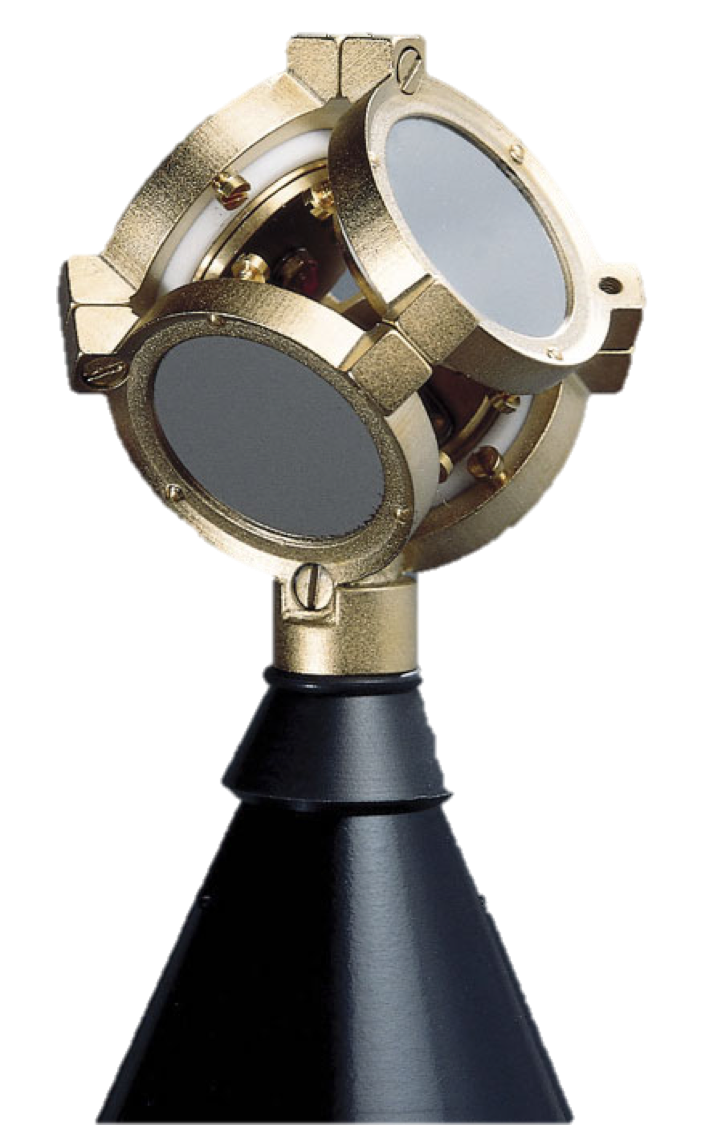
\includegraphics[scale = 0.3]{Sections/Background/images/soundFieldMic2.png}
			\end{minipage}
			\begin{minipage}{0.5\textwidth}
				\center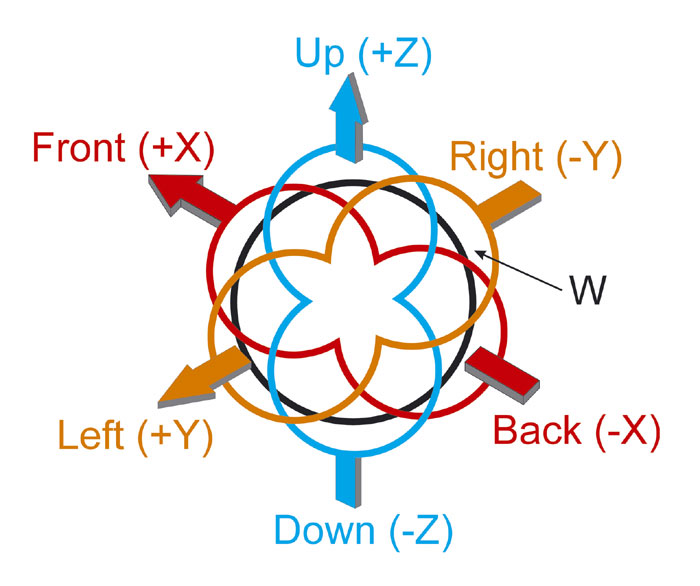
\includegraphics[scale = 0.3]{Sections/Background/images/soundFieldPolar.jpg}
			\end{minipage}
			\caption{\textbf{Left}: Picture of a Soundfield microphone with coincident capsules exposed. \textbf{Right}: Soundfield microphone polar pattern. Images sourced from~\cite{soundfieldMic} (background removed from left image) }
			\label{sfMic}
		\end{figure}

	\subsection{Software Overview}

		\subsubsection{Odeon: Simulating Room Acoustics}
		\label{Software:Odeon}

			%The techniques listen here are not used in this project and do not need to be fully understood. However they are mentioned for completeness and the use of them was considered at the start of the project and could be used in future work.
			Methods for physically measuring \ac{RIR}'s within rooms has been discussed, however there is also a way to synthesis \ac{RIR}'s by mathematical modelling the way in which sound interacts with a room. The two methods of doing so are described as \textbf{Wave-based Methods} and \textbf{Geometrical Acoustic Methods}.

			\textbf{Note: The next paragraph on wave-based methods is adapted from the initially submitted literature review and is not required for the understanding of this project. However, it is provided here as the initial project plan included the use of such methods and is therefore mentioned later in this section as well as \fullref{furtherwork}}

			Wave-based methods are based on solving the wave equation, producing a solution that is physically correct and can be used to accurately model how a sound would propagate from a source in a room and reflect \cite{Siltanen2010}. One such example is the finite-difference time-domain (FDTD) method, where sound is modelled by calculating the interaction between nodes in a rectangular mesh. The number of nodes in the mesh is determined by the frequency being modelled, therefore as the frequency being modelled increases, the number of nodes required in the mesh also increases which in turn increases computation time. It is for this reason that using wave-based methods are impractical for calculating high frequency sound propagation.

			Instead, it is possible to synthesis \ac{RIR}'s by using room acoustic simulation software such as Odeon \cite{odeon} that utilises the much quicker geometrical methods. Odeon was designed to provide reliable predictions of room acoustics by using a hybrid of two geometric acoustic modelling methods: \textbf{ray-tracing} and the \textbf{\ac{ISM}} to synthesis \ac{RIR}'s. These methods model how sound would propagate and interact with a room as though it were a straight line (ray). This inherently neglects wave phenomena such as phase and diffraction, properties that are negligible at high frequencies, however they are fundamental in describing low frequency wave behaviour \cite{Siltanen2010}. Therefore geometrical methods are not accurate at modelling sound propagation for low frequency waves, however they provide a good approximation for most applications and are much quicker to compute.

			A description of both of the geometrical methods are described below, leading to a description of the hybrid method used in Odeon.

		\paragraph{Ray-Tracing}
		\label{rayTracing}
			The ray-tracing method imitates a sound source by emitting a large number of particles in various directions from a single point \cite{Rindel1995}. These particles are then traced around the room,  losing energy each time the particle encounters a surface by a factor of $1 - \alpha$, where $\alpha$ is the absorption coefficient assigned to that surface, illustrated in figure~\ref{rayTracingImage}. The angle at which the particle is then reflected is determined by the scattering coefficient assigned to the surface of contact, ranging from a specular reflection to a completely random reflection \cite{odeonManual} (described in section~\fullref{background:scattering}). For a specific receiver position, an area around said point is defined in which rays are collected and used to calculate the results.

			\begin{figure}[H]
				\center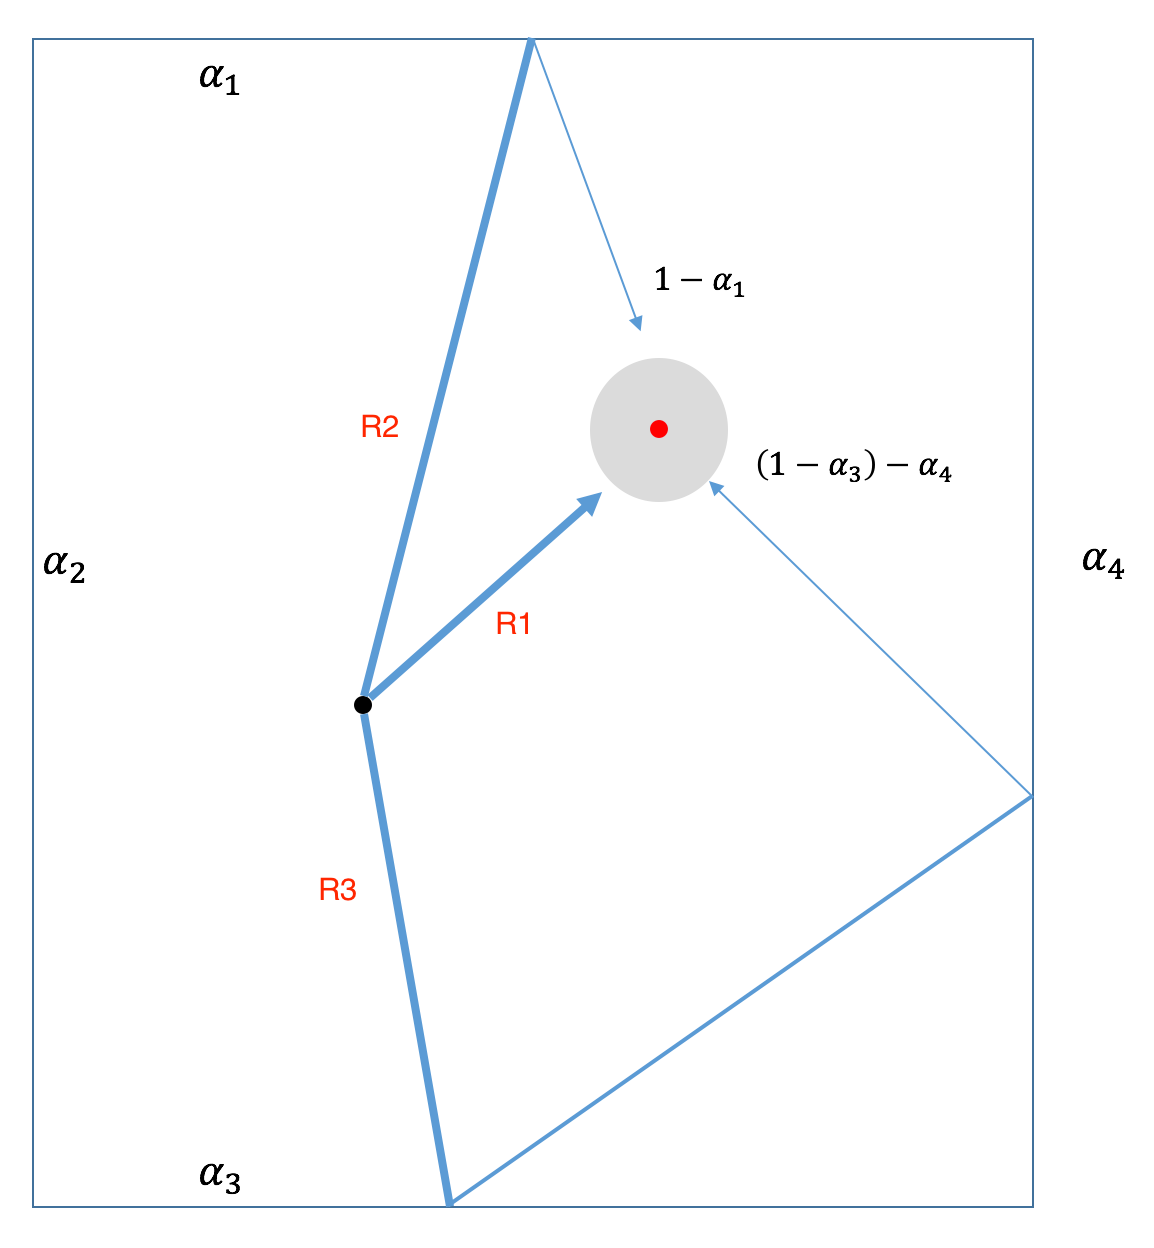
\includegraphics[scale = 0.5]{Sections/Background/images/rayTracingImage_edit.png}
				\caption{Illustration of the ray-tracing method (by the author) showing a sound source (black) emitting three rays (R1, R2 and R3) and shows how each ray is attenuated by a factor of $(1-\alpha$ each time it is reflected from a wall. The red dot represents the receiver positions and the outlining gray circle represents the area in which rays need to pass through to be used in the \ac{RIR} calculation.}
				\label{rayTracingImage}
			\end{figure}

			Ray-tracing does not provide a completely accurate result as it is a risk that some rays may not pass close enough to the receiver to contribute to the final result. The outcome of the ray-tracing method is a statistical result rather than a complete one.

		\paragraph{Image Source Method}

			%The \ac{ISM} represents specular reflections from surfaces as its own source, mirroring that of the original sound source, creating what is known as ``image sources'' \cite{Rindel1995} and can be used to find all possible specular reflection paths. Figure~\ref{ISMPic} illustrates this concept. The advantage of the \ac{ISM} is that each surface can be modelled by an image source which provides a great deal of data regarding the contribution to the received sound making this method more accurate than ray-tracing.

%			The \ac{ISM} can be used to find all possible specular reflections paths from the sound source to the receiver position. This is done by representing each specular reflection from a surface as a secondary source known as an ``image source'' \cite{Rindel1995}, illustrated in figure~\ref{ISMPic}. The advantage of the \ac{ISM} is that each surface can be modelled by an image source which provides a great deal of data regarding the contribution to the received sound as opposed to relying on random ray reflection as is done in the ray-tracing method, making this method more accurate, however as each image source then emits more rays, there is a possibility to produce a great deal more image sources. This means that the number of image sources grows exponentially for each new image source than is produced making this method much more computationally expensive than the ray-tracing method. This problem can be avoided by setting a \textit{reflection order} which determines how many times a ray can reflect off a surface before calculations are stopped, thus preventing the creation of more image source though the calculates for the prediction of the rooms acoustics will be incomplete. This obviously then makes the \ac{ISM} less accurate with a smaller reflection order.

			The \ac{ISM} can be used to find all possible specular reflection paths from the sound source to the receiver position. This is done by representing each specular reflection (a reflection with angle equal to the angle of incidence) from a surface as a secondary source known as an ``image source'' \cite{Rindel1995}, illustrated in figure~\ref{ISMPic}. Once these image sources have been created, a visibility test is run which checks to see which image sources are in sight of the receiver thus calculating which image sources should be used in the final calculation of the \ac{RIR}. If the receiver is then moved, the images sources to not need to be recalculated, only the visibility check needs to be run again. It is due to this that the \ac{ISM} is much more accurate than ray-tracing which relies on random reflections to calculate an \ac{RIR}. However, as each new image source emits a number of rays of its own, there is a potential for it to produce a number of image sources. Therefore, with each new image source there is an exponential growth in the total number of image sources, making this method much more computationally expensive than ray-tracing. This problem can be avoided by setting a \textit{reflection order} which determines how many times a ray can reflect around a room before calculations are stopped, thus preventing the creation of more image sources. This however will cause the prediction of the rooms acoustics to be incomplete. This obviously then makes the \ac{ISM} less accurate with a smaller reflection order.

			%Once all image sources have been calculated, a visibility check occurs. This checks to see whether the image sources that have been produced can be seen by the receiver, therefore checking whether that image source needs to be used or not offering the potential to cut down on computation time. If the receiver position is moved, the visibility check is run again. Overall, this saves time as the image sources do not need to be recalculated.


			\begin{figure}[H]
				\center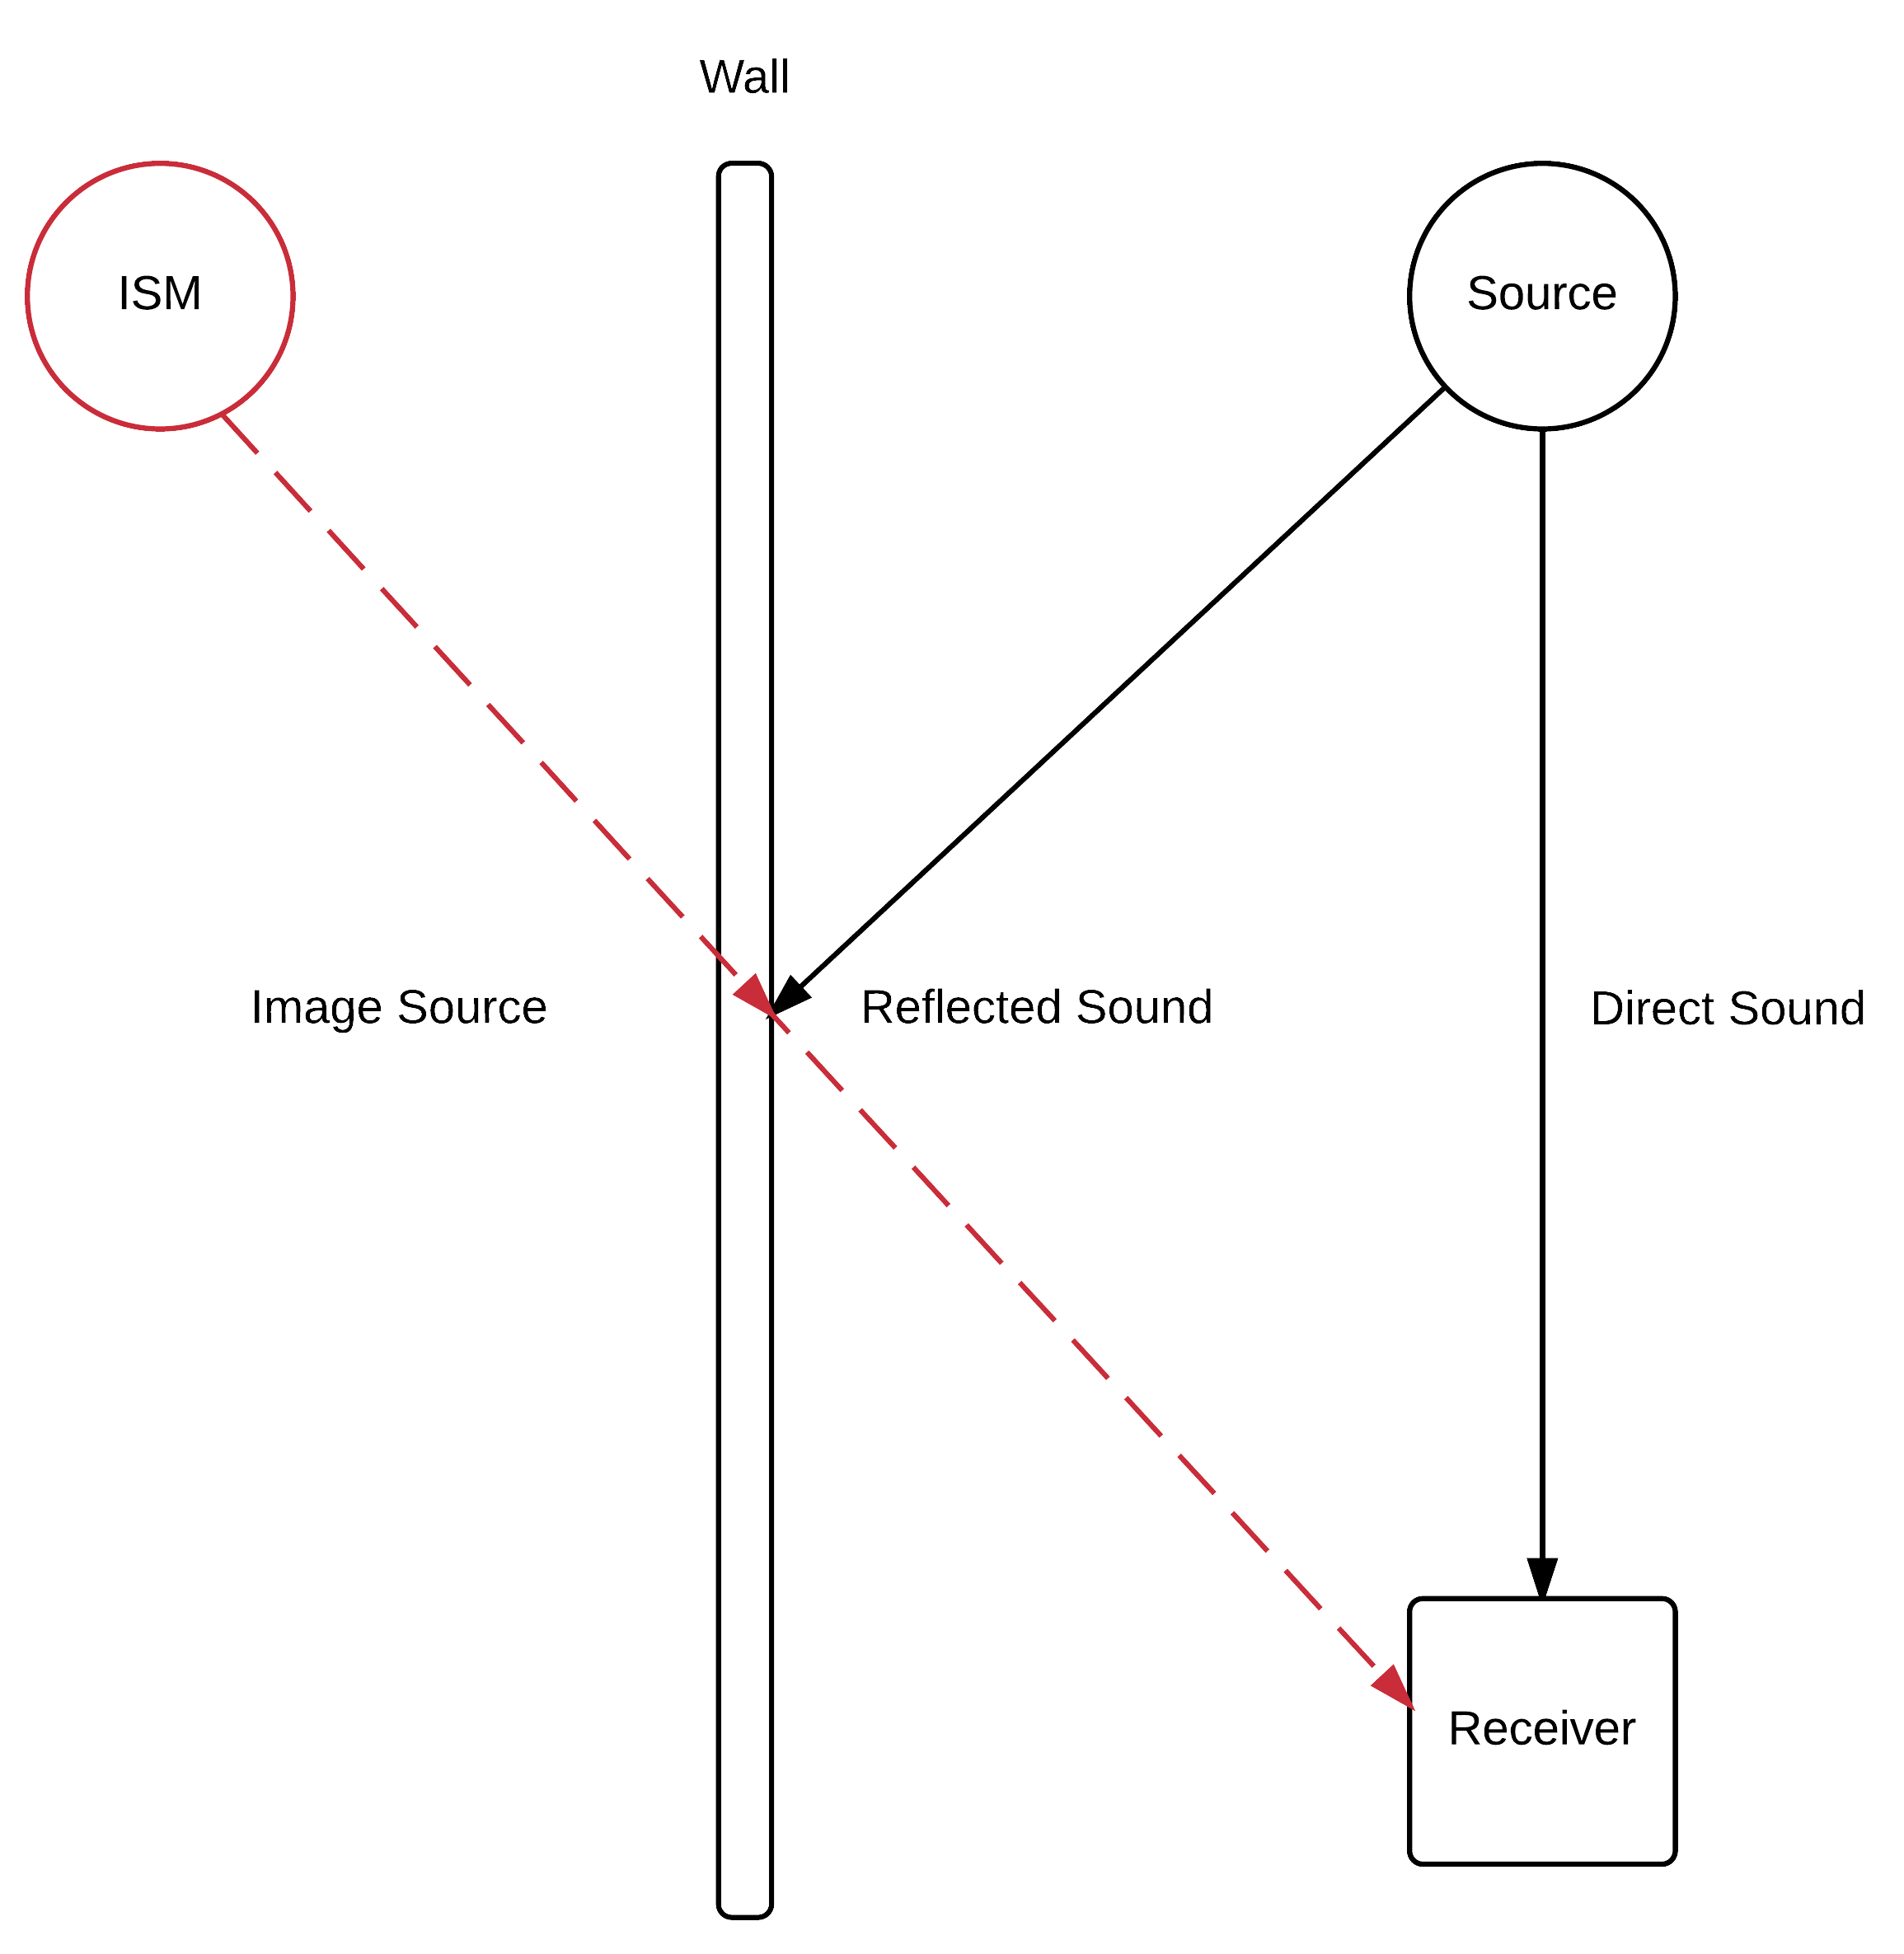
\includegraphics[scale = 0.4]{Sections/Background/images/ISM.png}
				\caption{Illustration of the image source method (by the author) showing how the reflection from the sound source to the receiver is modelled by a secondary sound source.}
				\label{ISMPic}
			\end{figure}

		\paragraph{Hybrid Method}
			%The inherent problems of the ray-tracing method and the \ac{ISM} are occluded by using a hybrid method that uses the best part of both. 

			Ideally, the \ac{ISM} would be used to calculate all sound rays due to its accurate results, however due to the computational limitations, Odeon uses a hybrid method to provide a reasonable compromise between calculation time and accuracy.

			The hybrid method first uses the \ac{ISM} to calculate a number of image sources up until a specified reflection order determined by a \ac{TO}. For example, if the \ac{TO} = 2, the image source method will allow a ray to reflect twice which will produce a number of image sources at which point it will then switch to using the ray tracing method to calculate a statistical model of how the rest of the rays might interact with the room. This gives the user the choice between computation time and accuracy.


		\paragraph{Scattering}
		\label{background:scattering}	

			Unless a surface is infinitely smooth (which almost all surfaces are not), when sound comes into contact with that surface it is scattered at a angle that deviates for that at which it hit the wall. Odeon takes this phenomena into account by using `Vector Based Scattering' \cite{odeonManual}. This is done by adding the specular vector to a randomly reflecting vector that has been scaled by a value of 1-s, where s is the scattering coefficient applied to a surface (ranging from 0 - 1). This essentially calculates how much a specular reflection should deviate based on how `rough' a surface is, where the rougher the surface, the higher the scattering coefficient. Figure~\ref{odeonScatterImage} shows an annotated image taken from the Odeon manual illustrating this concept.


			\begin{figure}[H]
				\center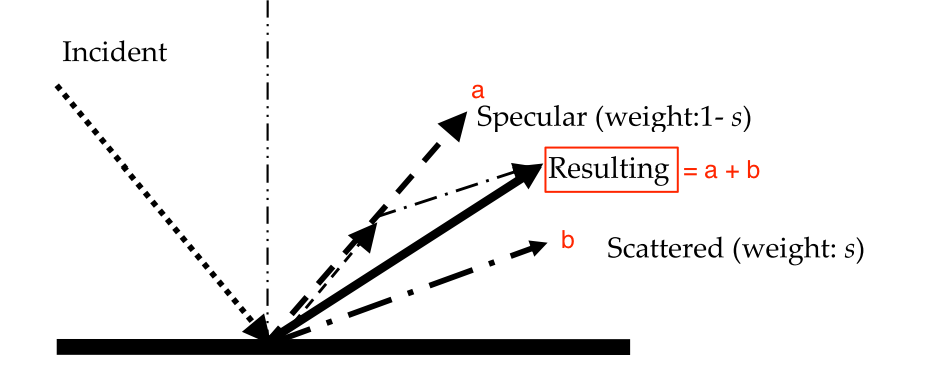
\includegraphics[scale = 1]{Sections/Background/images/scattering_edit.png}
				\caption{Annotated image from the Odeon manual \cite{odeonManual} showing how scattered reflections are calculated, where a = the specular reflection, b = randomly scattered vector.}
				\label{odeonScatterImage}
			\end{figure}

		\paragraph{Room Modelling}

			In order to predict the acoustics of a space, Odeon requires a geometry file in the form of a .par file. This file contains information regarding the room dimensions, object dimensions and positions. This can be produced within Odeon itself by using the built in `Extrusion Modeller' which allows a user to use a script like language to describe the rooms geometry. It is also possible to use 3rd party applications such as Google SketchUp \cite{SKU}, a software which is described in section~\fullref{GSU}.

		\paragraph{Material Selection}

			Selecting the appropriate absorption coefficients of the surfaces within a \ac{VAE} is crucial to determining how sound will attenuate as it reflects around the room (as described in \fullref{rayTracing}), thus the accuracy of the generated \ac{RIR}. Odeon provides a material list with common materials with pre-determined absorption coefficients that can be assigned to the surfaces of a model read from a geometry file. This material list can be extended by creating new materials and assigning absorption coefficients to the appropriate frequency bands.

	\subsubsection{Google SketchUp}\label{GSU}
		Google SketchUp \cite{SKU} is an easy to use 3-D modelling software that can be used to produce room models. Unlike Odeon extrusion modeller, it allows the user the draw surfaces with a mouse, easily duplicate structures and provides simple measuring tools and markers to enable accurate modelling. Plug-ins such as SU2Odeon (``SketchUp to Odeon'') \cite{SU2Odeon} enables the user to convert the model into a .par file for Odeon to use as a geometry file.

	\subsubsection{Max/MSP}
		Max/MSP (Max) is a visual programming language that essentially provides pre-written blocks of code in the form of objects, providing the ability to chain them together in order to route and manipulate audio signals \cite{max}. This allows user to quickly and easily produce audio applications (called patches) without having to deal with the complex side of audio programming. This is beneficial for students and researchers as it allows them to concentrate on the results rather than the application programming itself. Additionally, third-party plug-ins can be incorporated into a Max patch as libraries would in any other programming language. One third-party application utilised in this project is Spat. Developed at the research institute IRCAM \cite{spat}, Spat is designed for real-time spatialisation of sound signals in Max without having to touch any code. It provides a simple way to convolve B-format audio signals with impulse responses as well as decode the B-format signals for any given number of speakers in any arrangement by simply providing the number of speakers and angles at which they are placed.


\subsection{Project Description}
	
	This section starts by explaining what the \ac{VSS} is and how this project will build upon it. The motivation for doing so is covered and the project objectives and metrics are stated.

	\subsubsection{The Virtual Singing Studio}

		The \ac{VSS} is a loudspeaker based room acoustics simulator used as a tool for analysing the correlation between room acoustic characteristics and vocal performance parameters as part of Dr Jude Breretons PhD Thesis \cite{Brereton2014}. It is comprised of a head-mounted microphone used to capture a real-time audio input from a singer, a software patch written in Max/MSP that convolves the audio signal with a number of Ambisonic B-Format \ac{RIR}'s using Spat and finally a spherical array of 16 loudspeakers for which the convolved audio signals are decoded and sent. This allows the performer stood within the speaker array to hear themselves as though they are stood in the \ac{VAE}. In addition, a head-tracking device (an Oculus Rift \cite{oculus}) is also used to track which direction the user is facing in the virtual space. A flow diagram of the system is shown in figure~\ref{vssDiagram}.

	
		\begin{figure}[H]
			\centerline{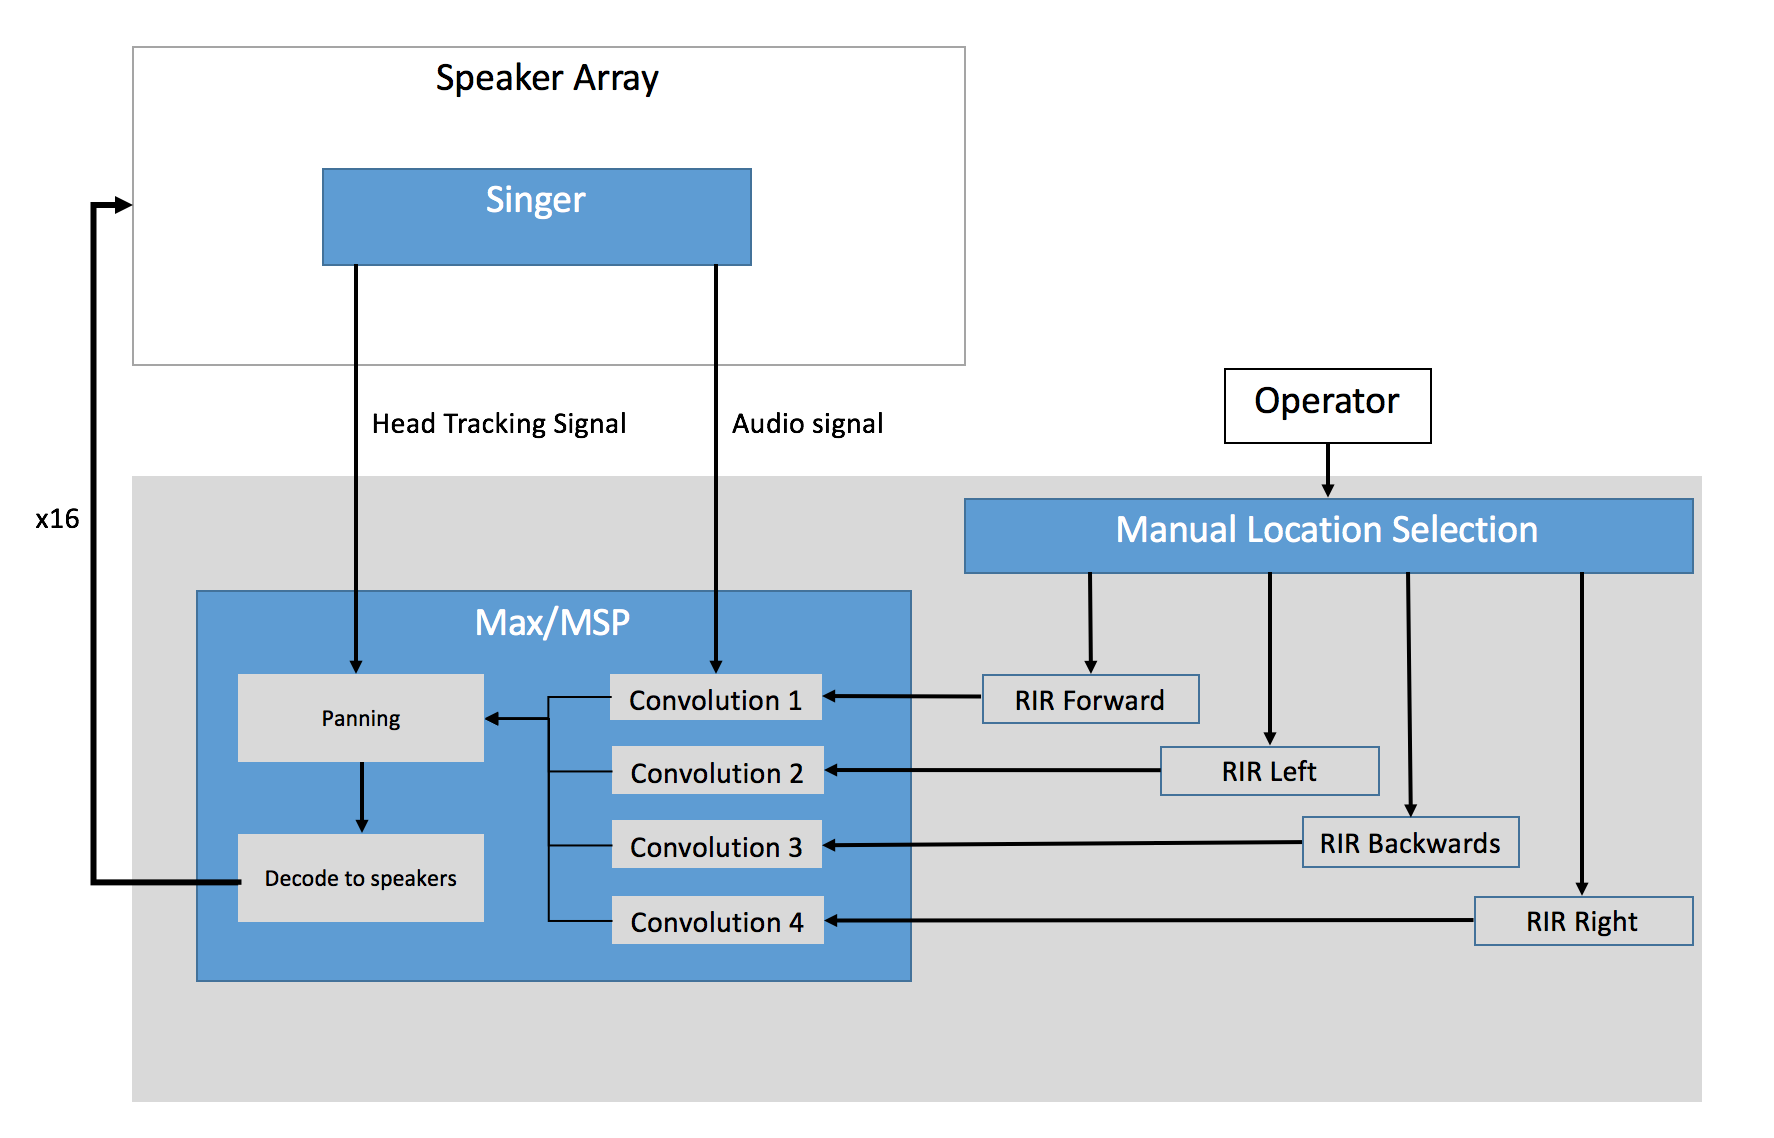
\includegraphics[scale = 0.45]{Sections/Background/images/vssDiagram.png}}
			\caption{Flow diagram of the VSS showing how the audio signal and head tracking signal from the performer are used in Max before the convolved audio signal is sent back out to the speaker array.}
			\label{vssDiagram}
		\end{figure}

		The \ac{VAE} used in the \ac{VSS} was initially the National Centre for Early Music, a space in York frequently used for musical performance. Using a Soundfield microphone, Ambisonic B-Format \ac{RIR}'s in each direction (front, left, back, right) were captured in 4 locations. The four directional \ac{RIR}'s are used to approximate the room acoustic phenomena that would occur if the user were projecting whatever sound they are producing in that direction. This is done by using the data from the head-tracking device to amplitude pan the convolved signals before sending them to the spherical speaker array.


	\subsubsection{Project Aims and Motivation}
	\label{background:aims}
		
		The \ac{VSS} addressed a problem faced when trying to research how musicians perform in different acoustic environments: having to travel to each performance space with musicians and researchers. This also indirectly provides a solution for performers wanting to rehearse in spaces that are often inaccessible and would otherwise be expensive to book and travel to. By obtaining an \ac{RIR} of the desired location, the only time travelling will be necessary is to initially obtain said \ac{RIR}. However, one limitation of using the \ac{VSS} is the restriction of position. If a performer wanted to try and sing at another point in the room, an \ac{RIR} would have to be taken in that position too. This could be done initially, taking a range of \ac{RIR}'s in a number of positions, however it cannot be guaranteed that all positions desirable to the performer will be available. For this to be certain, technically an infinite number of \ac{RIR}'s would have to be taken. As this is obviously not possible, the next best thing would be to take a large grid of \ac{RIR}'s and simulate movement by interpolation between a number of neighbouring \ac{RIR}'s. This raises the question:



		 \vspace{5mm}
		 \begin{center}
		 \begin{minipage}{0.7\textwidth}
		 How many \ac{RIR}'s are required to convince a user that they are able to move to any position they like within the virtual space?
		 \end{minipage}
		 \end{center}
		 \vspace{5mm}


		 As investigating this question would require producing a large grid of \ac{RIR}'s, measuring them in a real space would be impractical due to the sheer number that need to be taken for experimentation. Instead, Odeon can be used to produce a bulk of \ac{RIR}'s much quicker.

		This technique has been considered previously in \cite{Savioja1999}, referring to it as the \textit{direct room impulse response rendering method}. However another method called \textit{parametric room impulse response rendering} was favoured instead. This method actually synthesises \ac{RIR}'s in real time for a given position of the user within a \ac{VAE} using geometric acoustic modelling methods. The reason this was chosen over the dynamic method was the fact that rendering the \ac{RIR} for the users virtual position would be much more accurate and would not require storage space, as opposed to having to interpolate between a number of \ac{RIR} that have to be stored somewhere. However, this method is much more complicated and limits itself to the accuracy of geometrical methods as wave-based methods are currently not able to run in real time (not even with using GPU technology, still taking approximately 10 minutes to render a single \ac{RIR} \cite{Mehra2010}).

		There are three reasons why using the direct rendering method in this project was initially considered: 
		\begin{enumerate}
			\item Simplicity, as a real time \ac{RIR} rendering system would not have to be produced.
			\item The existing \ac{VSS} system could be used as a starting point (thus adding to the simplicity).
			\item The potential to use wave-based methods.
		\end{enumerate}

		As using the parametric method requires the \ac{RIR}'s to be calculated in real time, it would not be possible with current technology to produce a more accurate \ac{RIR} than can be obtained using the geometrical acoustic modelling methods. However, as the direct \ac{RIR} method produces the \ac{RIR}'s offline, it could be possible be produce more accurate results. This has been investigated previously \cite{Oxnard2013}, where the \ac{RIR}'s calculated in Odeon are merged with the low-frequency accurate \ac{RIR}'s calculated using wave-based methods to produce an accurate full bandwidth \ac{RIR} using calibration methods (a method to accurately mix the two together) proposed in \cite{Southern}. However, early in the project it was decided that using wave-based modelling methods would be much too time consuming to implement along with carrying out the primary project aims given 1) the time scale of the project and 2) the time it takes to produce such \ac{RIR}'s compared to the ones produced in Odeon. It was therefore decided that a system would be built using only \ac{RIR}'s produced in Odeon which would still allow the question of how many \ac{RIR}'s are required to produce such a system to be investigated.

		% The author stated:

		%  \vspace{5mm}
		%  \begin{center}
		%  \begin{minipage}{0.5\textwidth}
		%  \textit{``Although a static setting would be technically much simpler, it has only limited applicability''}
		%  \end{minipage}
		%  \end{center}
		%  \vspace{5mm}

	
		% It can be said that although parametric room impulse response rendering might be limited in its applicability, for the aims of the project described in this document, it provides a solution that is simple enough to implement within the time given and will allow for the desired functionality. It will also be explained later in this document (\fullref{RIRtrimming}) that post-processing of the \ac{RIR}'s are required which would not be possible using the dynamic rendering method. Therefore, as the intention was to build upon the existing \ac{VSS} system which requires pre-recorded (and post-processed) \ac{RIR}'s and that storage space is no longer a problem due to cheap hard disc drive storage, it was decided that the direct room impulse response rendering method was to be used. In addition to implementing the desired functionality, the following additional information were to be investigated:

		
		% 	\textbf{The process:} Given the apparent simplicity compared to producing a dynamic rendering system, the process of obtaining the \ac{RIR}'s was to be accessed.

		% 	\textbf{Number of \ac{RIR}'s:} As one of the points mentioned was the space required to store the \ac{RIR} grid(s), the number of \ac{RIR}'s required to convince the user that they are moving freely around the virtual space was to be investigated.

		% 	\textbf{System authenticity:} Previous test in the VSS have required ‘plausibility’ test, where the user must evaluate the \ac{VAE} produced by the VSS without reference to the real venue. This is usually because testing a virtual environment against a real one (authenticity tests) requires travel which can be expensive and difficult. Therefore, by running test based on ‘plausibility’ a sense of how convincing the virtual room is can be obtained. In the case of other virtual reality systems where the virtual environment does not exist in the real world, only these types of test can be run. Though plausibility test are acceptable, an authenticity test gives more objective results by comparing the simulated \ac{VAE} to the real thing. Therefore impulse responses of the same room used to designed the \ac{VAE} were to be taken.

		%As mentioned in section~\ref{Software:Odeon}, using geometrical acoustic modelling methods produce \ac{RIR}'s that do not produce accurate low frequency content. Therefore, it was decided to seize the opportunity to test the authenticity of the system.

		

		In order for the user to move themselves around the \ac{VAE}, the Max patch that the \ac{VSS} was built on had to be extended in the following ways:

		\begin{enumerate}

			\item The production of a user interface that can be used remotely from within the spherical speaker array. \\

			\item The extension of the Max patch that could accommodate the user interface and load the appropriate \ac{RIR} files required to place the user in the desired location within the \ac{VAE}. \\

			\item The production of a system that can interpolate between the appropriate \ac{RIR} positions.

		\end{enumerate}

		Figure~\ref{vssExtention} shows an adapted flow diagram from figure~\ref{vssDiagram} with the added user interface and automatic file searching functionality.

		\begin{figure}[H]
			\centerline{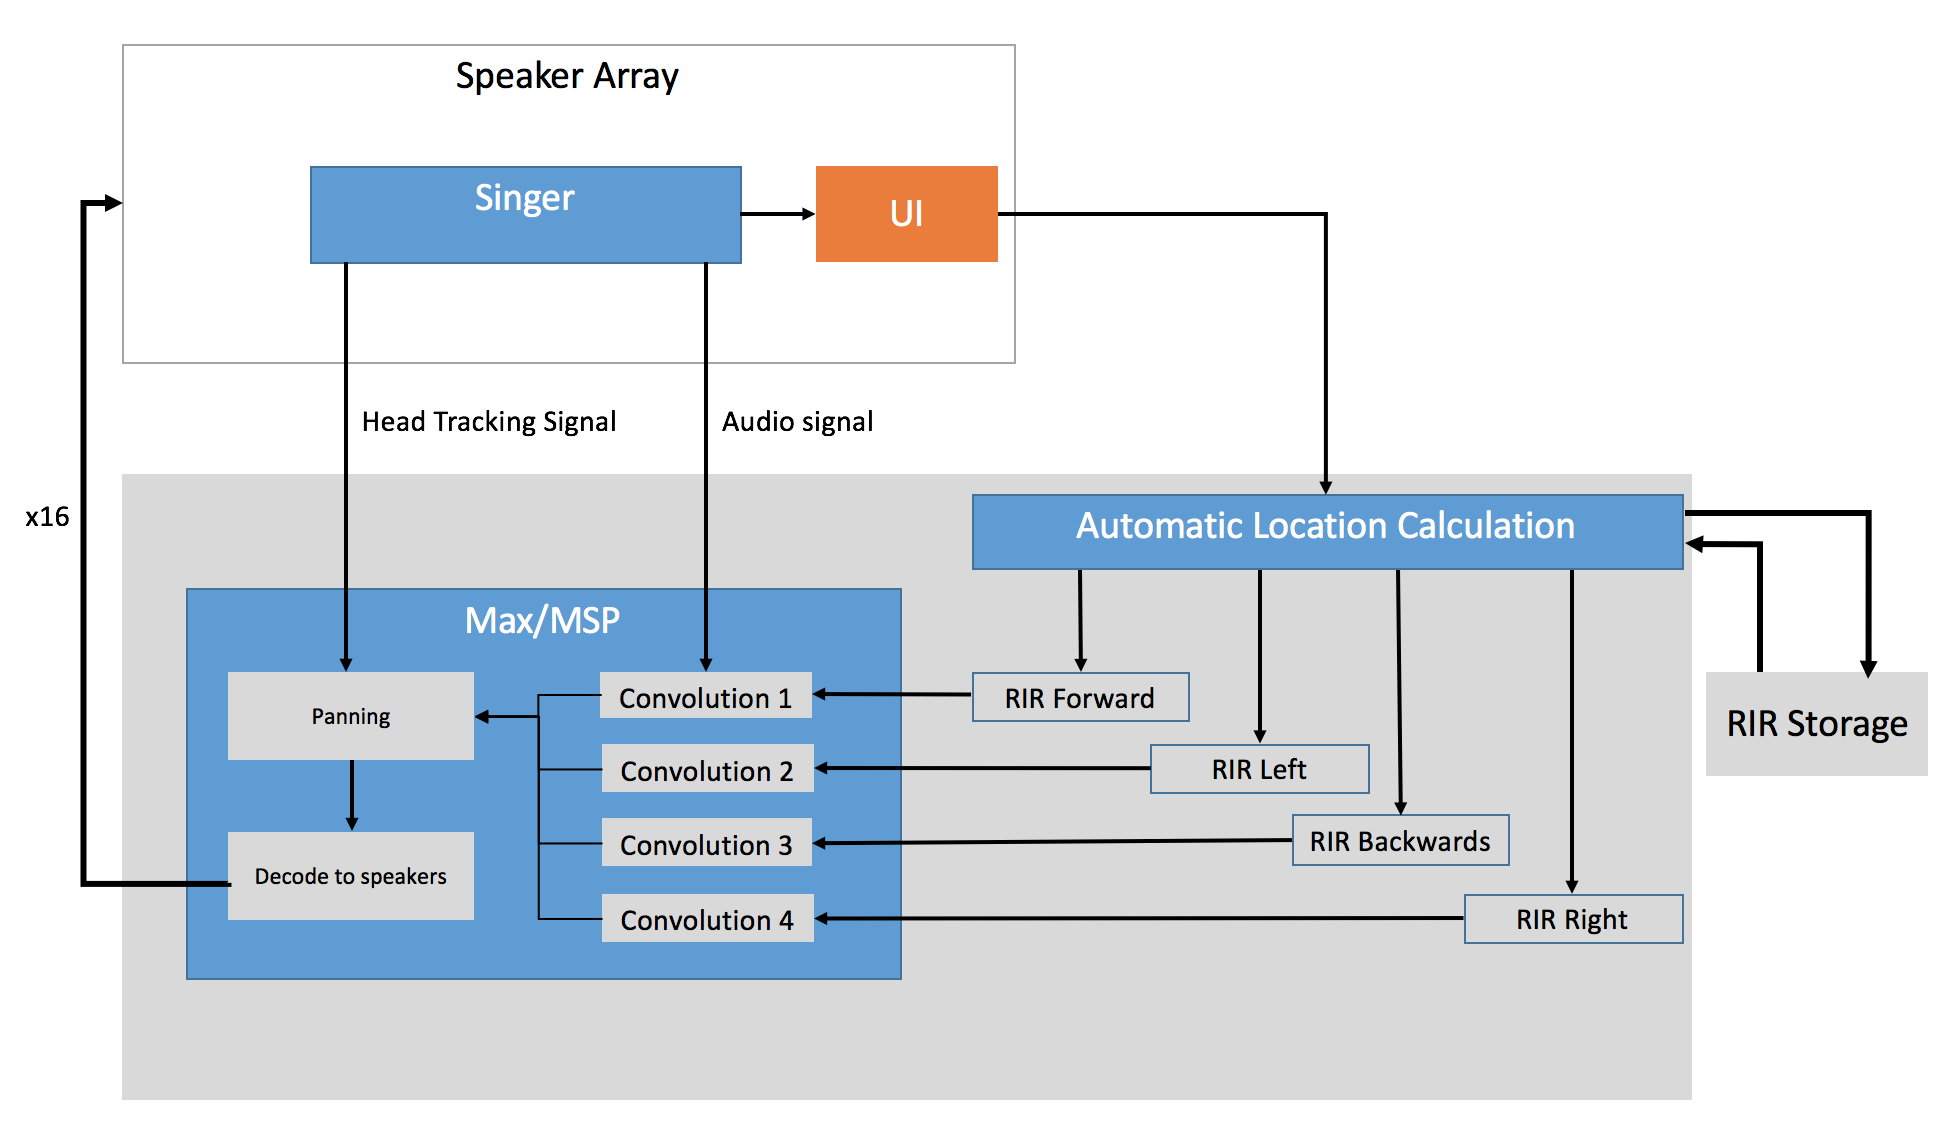
\includegraphics[scale = 0.45]{Sections/Background/images/vssExtention.png}}
			\caption{Flow diagram of the way in which the desired extended version VSS works}
			\label{vssExtention}
		\end{figure}

		As the original implementation of the \ac{VSS} uses real \ac{RIR}'s to simulate a \ac{VAE} and the newly proposed implementation was to use synthetic \ac{RIR}'s, the difference in perception regarding how a user feels they are moving around the space was also to be investigated. This would provide an insight as to whether the newly implemented functionality of movement was worth sacrificing the accuracy of the real \ac{RIR}'s. For this to be investigated, real \ac{RIR} measurements must be taken, therefore, the \ac{VAE} to be modelled must be a building that was accessible for real \ac{RIR} measurements.

		To conclude, the project aims were:

		\begin{enumerate}
			\item To implement a direct \ac{RIR} rendering system as an extension of the \ac{VSS}

			\item To investigate the number of \ac{RIR}'s that are required to convince a user that they can freely move themselves around a virtual space without limitation

			\item To investigate the difference in the perception of mobility in the virtual space when using real \ac{RIR}'s and synthetic \ac{RIR}'s
		\end{enumerate}

	\subsubsection{Project Objectives}
	\label{background:objectives}

		Given the project aims and the background provided, the following is a list of objectives that were set in order to complete this project:

		\begin{enumerate}
			\item Find an appropriate room to be modelled as a \ac{VAE} 
			\item Digitally model the room using in Google SketchUp
			\item Import room model into Odeon to finish material selection and \ac{RIR} settings
			\item Produce a grid of \ac{RIR}'s that can be used to interpolate between to simulate user positions
			\item Record real \ac{RIR}'s in locations that can be compared to synthetic \ac{RIR}'s
			\item Extend upon existing software patch to accommodate new functionality
			\item Preform user tests:
				\begin{itemize}
					\item Test \#1: Does the perception of distance change when using real or synthetic \ac{RIR}'s?
					\item Test \#2: How far does the user have to move in the given \ac{VAE} before they notice they have moved 
					\item Test \#3: How many \ac{RIR}'s are required for interpolation for the user to feel they are moving around the space freely
				\end{itemize}
			\end{enumerate}


	% To assess the success of this project, the following list of statements are defined with the intent of evaluating the extent of their correctness:


	% Upon completion of the project, the answers to the following questions can be used to evaluate the success of the project 

	% \begin{itemize}
	% 	\item Was the above described system full implemented?
	% 	\item Was the number of \ac{RIR}'s required to produce the system discovered?
	% 	\item 
	% \end{itemize}

	% \begin{itemize}
	% 	\item Produce a system that:
	% \begin{itemize}
	% 	\item[-] Allows the user to move themselves around the \ac{VAE} freely
	% 	\item[-] Is beneficial to the user
	% 	\item[-] Is simple to implement compared to other methods
	% \end{itemize}

	% 	\item Obtain information regarding:
	% 	\begin{itemize}
	% 		\item[-] How many \ac{RIR}'s are required for convincing mobility
	% 		\item[-] The effect of using synthetic \ac{RIR}'s on the perception of movement
	% 	\end{itemize}
	% \end{itemize}

\end{document}